\chapter{Google Dialogflow}

Dialogflow\cite{dialogflow} is a platform developed by Google to build natural and rich conversational experiences. Much like the Microsoft's Botframework, Dialogflow aims to make it possible for chatbot creators to create a single chatbot that connects to multiple channels like Skype, Slack and Messenger, etc.

Dialogflow seems to focus on the usage of their GUI and tools to create conversations, but it's also possible to write all of the logic using code.

\section{Business Model}

Google offers 2 main pricing options for their platform. Firstly there is the free edition, it includes free usage with unlimited text query requests. These requests are limited to 3 queries per second. It's also possible to easily integrate voice interaction into Dialogflow, the free edition limits these kinds of interactions to 1000 requests per day with a maximum of 15000 per month. Support is also limited to community and email support. Google themselves recommend this plan for small to medium businesses or developers trying to experiment with Dialogflow. Next to the free edition, there is an enterprise edition as well. This edition has a pay as you go model, which means it's easily scalable as the business will be paying per request. Choosing this option also opens up the possibility to integrate Google Cloud Support and receive specialized instant support.

\section{Technical implementation}

Because Dialogflow is very focused on their GUI, small to medium businesses that don't need extensive logic in their chatbot can make use of the existing tools to create a chatbot. This is recommended to get started and get familiar with the platform. When more complicated logic needs to be implemented like API calls and custom logic that wouldn't be supported by the platform, custom \Gls{Webhook}s can be created. These allow developers to receive a message that was recognized by Dialogflow and implement their custom logic to handle the message.

It's also possible to take full advantage of Dialogflow using their client libraries. These libraries are available for C\#, GO, Java, Node.JS, PHP, Python and Ruby. There is some documentation available to get started but diving deeper into the development will take great effort. To take advantage of this functionality, the enterprise edition of Dialogflow needs to be used.

\subsection{Developer environment}

There are several ways to choose a development environment and set up a workflow. Using Google Dialogflow isn't just focused on coding, developers mostly need to work with the user interface provided by google.

To get started, simply making use of the website GUI will suffice. There is also an inline editor~\ref{fig:dialogflow-inline-editor} provided to handle requests in code. Another way to handle requests is by enabling a custom webhook to receive information from Dialogflow, like an intent that was recognized, and handle it. This webhook would be written by the developer, following Dialogflow's specification to send back messages. Setting up this webhook is completely up to the developer, it can be done in any server language and does not make use of any library linked to Dialogflow, all the webhook will receive is a simple POST request.

\begin{figure}[ht]
	\centering
	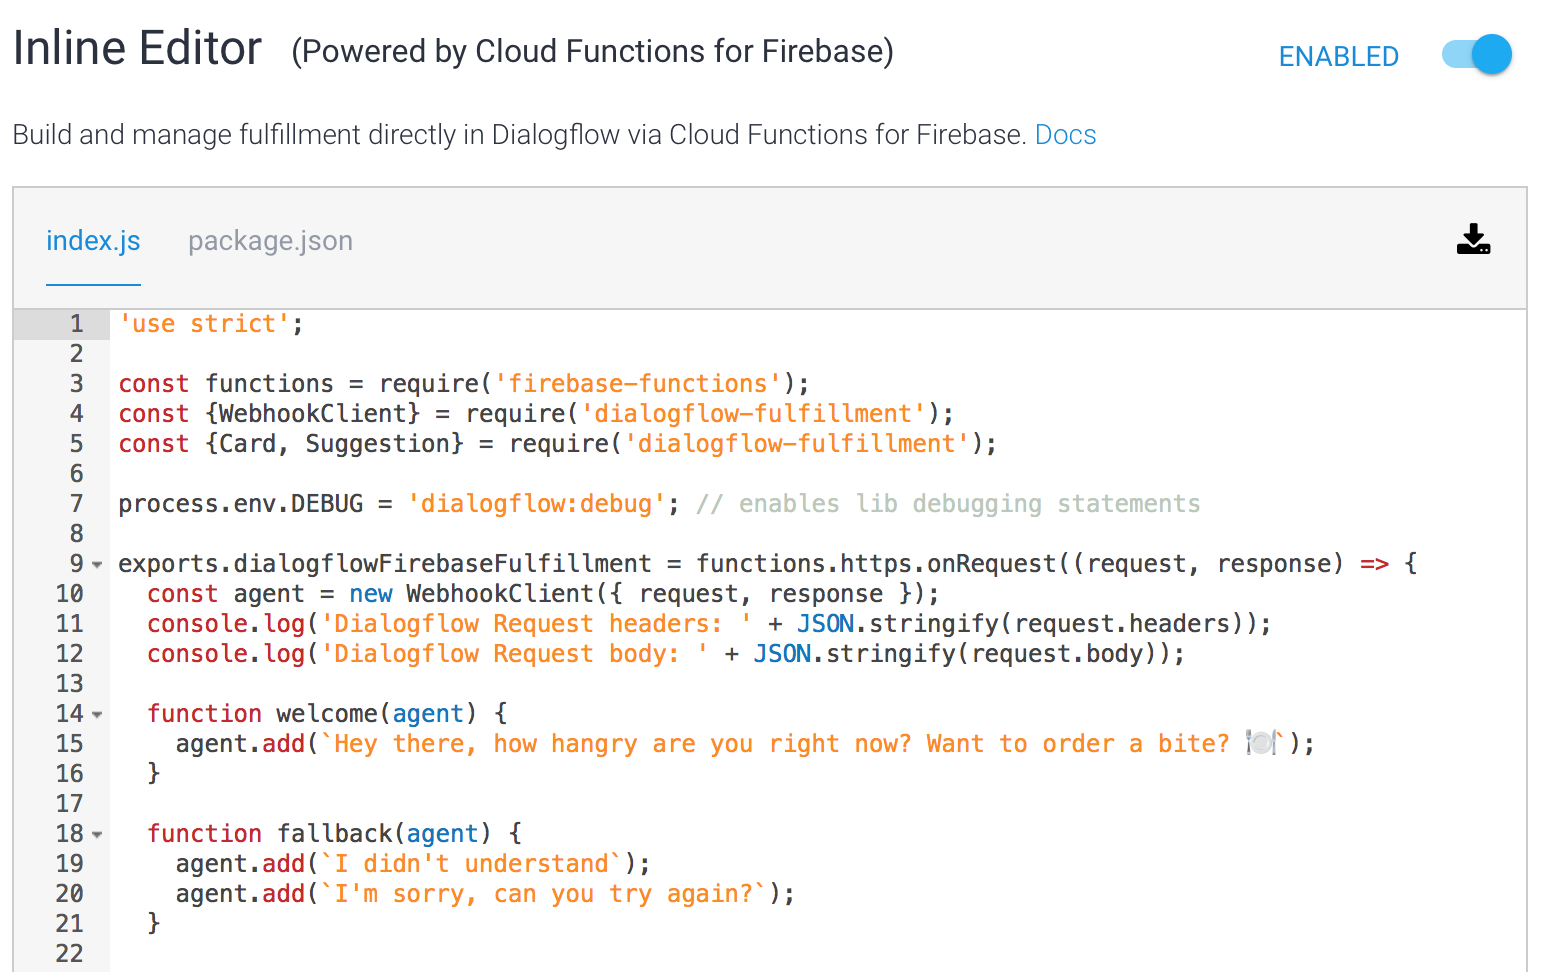
\includegraphics[width=0.8\textwidth]{dialogflow-inline-editor}\label{fig:dialogflow-inline-editor}
	\caption{Dialogflow's inline editor for handling intents}
\end{figure}

\subsection{Testing}

\begin{wrapfigure}{r}{0.35\textwidth}
	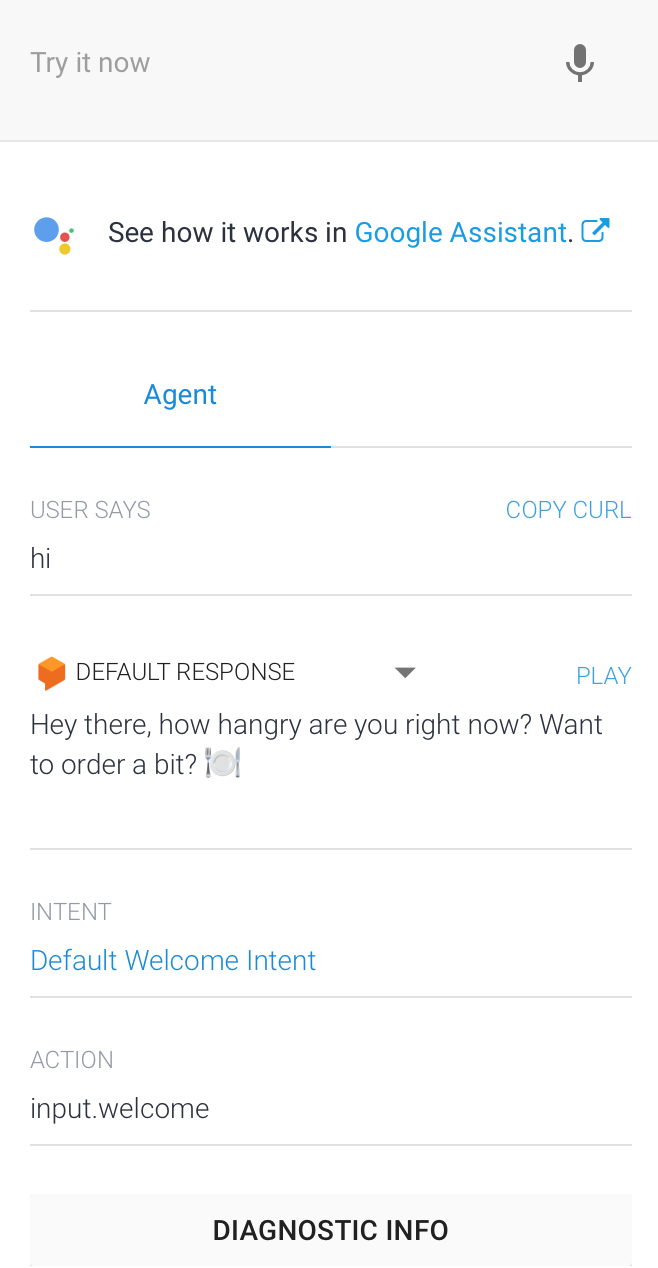
\includegraphics[width=0.7\linewidth]{dialogflow-testing}\label{fig:dialogflow-testing}
	\caption{Testing a bot using the Dialogflow platform}
\end{wrapfigure}

Testing the bot is done using Dialogflow's own testing segment on the interface. When making use of a custom webhook testing becomes more complicated as the webhook will have to be deployed every time the developer wants to actually test the replies of the chatbot.

\newpage

\section{Building a bot}

\section{Constructing a conversational flow}